\documentclass[a4paper,11pt,dvipdfmx]{jsarticle}


% 数式
\usepackage{amsmath,amsfonts,amssymb,amsthm}
\usepackage{bm}
\usepackage[version=4]{mhchem}
\usepackage{color}
% 画像
\usepackage[dvipdfmx]{graphicx}
\usepackage{tikz}
\usetikzlibrary{intersections,calc,arrows.meta}
\usepackage{ascmac}
\usepackage{url}

\begin{document}

\section*{各式の証明, 説明}
授業中に先生に説明を求められた数式や原理などの説明をまとめる。
\begin{enumerate}
  \item 外積の計算公式
  \begin{align*}
    \nabla \cdot (\mathbf{A} \times \mathbf{B}) = \mathbf{B} \cdot (\nabla \times \mathbf{A}) - \mathbf{A} \cdot (\nabla \times \mathbf{B})
  \end{align*}
  を完全反対称テンソルを使って証明する。なお、$\mathbf{A} = (A_i, A_j, A_k), \mathbf{B} = (B_i, B_j, B_k)$とする。
  \begin{itembox}[l]{完全反対称テンソルとは}
    3次元における完全反対称テンソルは、以下のように定義される。
    \begin{align*}
      \epsilon_{ijk} = 
      \begin{cases}
        1 &  (i, j, k), (k, i, j), (j, k, i) \\
        -1 &  (i, k, j), (k, j, i), (j, i, k) \\
        0 & その他
      \end{cases}
    \end{align*}
    右側のカッコは、添字の順番を表している。つまり$ijk$の順番であれば1であり、いずれかの文字を1回入れ替えると$-1$になる。そこから更に1回入れ替えると1に戻る。
    \\
    \textbf{参考URL}: \url{https://mashiroyuya.hatenablog.com/entry/levicivitasymbol_delta}
  \end{itembox}
  \begin{proof}[\textbf{証明}]
    完全反対称テンソルを用いることで、外積の式は以下のように書くことが可能である。
    \begin{align*}
      \frac{\partial}{\partial r_i}\left( \epsilon_{ijk} A_j B_k \right) &= \epsilon_{ijk}\left( \frac{\partial}{\partial r_i} A_j B_k + A_j \frac{\partial}{\partial r_i} B_k \right) 
      \\
      &= \epsilon_{kij}\frac{\partial}{\partial r_i}A_j B_k - \epsilon_{jik}A_j \frac{\partial}{\partial r_i}B_k
    \end{align*}
    変形後の右辺第一項は
  \end{proof}
  
  \item マクスウェル方程式から導出された2式
  \begin{align*}
    \begin{cases}
      \nabla \times \mathbf{E}(\mathbf{r}) - i \omega \mu_0 \mathbf{H}(\mathbf{r}) = 0 \cdots  (1) \\
      \nabla \times \mathbf{H}(\mathbf{r}) + i \omega \epsilon_0 \epsilon(\mathbf{r})\mathbf{E}(\mathbf{r}) = 0 \cdots (2)
    \end{cases}
  \end{align*}
  から、マスター方程式を導出する。
  \begin{proof}[\textbf{導出過程}]
    (2)式の両辺を$\epsilon(\mathbf{r})$で割って、curl(rot)をとり、(1)式を代入する。
    \begin{align*}
      &\qquad \frac{1}{\epsilon(\mathbf{r})} \nabla \times \mathbf{H(r)} + i \omega \epsilon_0 \mathbf{E(r)}
      \\
      & \Longleftrightarrow \nabla \times  \left( \frac{1}{\epsilon(\mathbf{r})} \nabla \times \mathbf{H(r)} + i \omega \epsilon_0 \mathbf{E(r)} \right) = 0 \\
      & \Longleftrightarrow \nabla \times  \left( \frac{1}{\epsilon(\mathbf{r})} \nabla \times \mathbf{H(r)} \right) + \nabla \times \left( i \omega \epsilon_0 \mathbf{E(r)}  \right)= 0 \\
      & \Longleftrightarrow \nabla \times  \left( \frac{1}{\epsilon(\mathbf{r})} \nabla \times \mathbf{H(r)} \right) + i \omega \epsilon_0 \nabla \times \mathbf{E(r)} = 0 \\
      & \Longleftrightarrow \nabla \times  \left( \frac{1}{\epsilon(\mathbf{r})} \nabla \times \mathbf{H(r)} \right) - \omega^2 \epsilon_0 \mu_0 \mathbf{H(r)} = 0 \\
    \end{align*}
    $\displaystyle c^2 = \frac{1}{\epsilon_0 \mu_0}$の変換を行い、式を整理すると
    \begin{align*}
      \nabla \times  \left( \frac{1}{\epsilon(\mathbf{r})} \nabla \times \mathbf{H(r)} \right) = \left( \frac{\omega}{c} \right)^2 \mathbf{H(r)}
    \end{align*}
  \end{proof}
  \item 内積計算の公式($(F, \hat{\Theta}G) = (\hat{\Theta}F,G)$)を証明する
  % // TODO:
  \item 
    \begin{align*}
      \begin{cases}
        \displaystyle
        u_f (\mathbf{H} + \delta \mathbf{H}) = \frac{(\mathbf{H} + \delta \mathbf{H}, \hat{\Theta}\mathbf{H} + \hat{\Theta}\delta \mathbf{H})}{(\mathbf{H} + \delta \mathbf{H}, \mathbf{H} + \delta \mathbf{H})} \\
        \displaystyle
        u_f (\mathbf{H}) = \frac{(\mathbf{H}, \hat{\Theta}\mathbf{H})}{(\mathbf{H}, \mathbf{H})} \\
        \delta u_f (\mathbf{H}) \triangleq u_f(\mathbf{H} + \delta \mathbf{H}) - u_f(\mathbf{H})
      \end{cases}
    \end{align*}
    以上3式より、$\delta u_f (\mathbf{H}) \thickapprox \left[ (\delta \mathbf{H}, \mathbf{G}) + (\mathbf{G}, \delta\mathbf{H}) \right] / 2$のように表せることを証明する。

    \begin{proof}[\textbf{導出過程}]
      \begin{align*}
        (\mathbf{H} + \delta \mathbf{H}, \mathbf{H} + \delta \mathbf{H}) &= (\mathbf{H}, \mathbf{H}) + (\mathbf{H}, \delta \mathbf{H}) + (\delta \mathbf{H} , \mathbf{H}) ((\delta \mathbf{H}, \delta \mathbf{H})は2次の微小項なので無視) \\ 
        &= (\mathbf{H}, \mathbf{H}) \left( 1 + \frac{(\mathbf{H}, \delta \mathbf{H}) + (\delta \mathbf{H}, \mathbf{H})}{(\mathbf{H}, \mathbf{H})} \right)
      \end{align*}
      よって、$ u_f(\mathbf{H} + \delta \mathbf{H})$は、以下のように変形することが可能。2行目でカッコの外側の分数の第二項において、$\hat{\Theta}$を移していることに注意。また、テイラー展開を用いていることにも注意。
      \begin{align*}
        u_f (\mathbf{H} + \delta \mathbf{H}) &= \cfrac{(\mathbf{H}, \hat{\Theta}\mathbf{H}) + (\mathbf{H}, \hat{\Theta}\delta\mathbf{H}) + (\delta \mathbf{H}, \hat{\Theta}\mathbf{H}) }{(\mathbf{H}, \mathbf{H}) \left( 1 + \cfrac{(\mathbf{H}, \delta \mathbf{H}) + (\delta \mathbf{H}, \mathbf{H})}{(\mathbf{H}, \mathbf{H})} \right)}
        \\ 
        &= \cfrac{(\mathbf{H}, \hat{\Theta}\mathbf{H}) + (\hat{\Theta}\mathbf{H}, \delta\mathbf{H}) + (\delta \mathbf{H}, \hat{\Theta}\mathbf{H}) }{(\mathbf{H}, \mathbf{H})} \left( 1 - \cfrac{(\mathbf{H}, \delta \mathbf{H}) + (\delta \mathbf{H}, \mathbf{H})}{(\mathbf{H}, \mathbf{H})} \right)
      \end{align*}
      よって、$\delta u_f (\mathbf{H})$は、
      \begin{align*}
        \delta u_f (\mathbf{H}) &= u_f(\mathbf{H} + \delta \mathbf{H}) - u_f (\mathbf{H}) \\
        &= \cfrac{(\mathbf{H}, \hat{\Theta}\mathbf{H}) + (\hat{\Theta}\mathbf{H}, \delta\mathbf{H}) + (\delta \mathbf{H}, \hat{\Theta}\mathbf{H}) }{(\mathbf{H}, \mathbf{H})} \left( 1 - \cfrac{(\mathbf{H}, \delta \mathbf{H}) + (\delta \mathbf{H}, \mathbf{H})}{(\mathbf{H}, \mathbf{H})} \right) - \frac{(\mathbf{H}, \hat{\Theta} \mathbf{H})}{(\mathbf{H}, \mathbf{H})} \\
      \end{align*}
      ここで、$(\hat{\Theta}\mathbf{H}, \delta \mathbf{H})  (\mathbf{H}, \delta \mathbf{H})と (\delta \mathbf{H}, \hat{\Theta}\mathbf{H})  (\delta\mathbf{H}, \mathbf{H})$は2次の微小項なので無視すると、
      \begin{align*}
        \delta u_f &= \cfrac{(\hat{\Theta}\mathbf{H}, \delta\mathbf{H}) + (\delta \mathbf{H}, \hat{\Theta}\mathbf{H}) }{(\mathbf{H}, \mathbf{H})} - \cfrac{(\mathbf{H}, \delta \mathbf{H}) + (\delta \mathbf{H}, \mathbf{H})}{(\mathbf{H}, \mathbf{H})^2}(\mathbf{H}, \hat{\Theta}\mathbf{H})
      \end{align*}
      
      以上の式を整理して、
      \begin{align*}
        \mathbf{G}(\mathbf{H}) = \frac{2}{(\mathbf{H}, \mathbf{H})}\left( \hat{\Theta}\mathbf{H} - \left[ \frac{(\mathbf{H}, \hat{\Theta}\mathbf{H})}{(\mathbf{H}, \mathbf{H})} \right] \mathbf{H} \right)
      \end{align*}
      と定義することで、$\delta u_f (\mathbf{H}) \thickapprox \left[ (\delta \mathbf{H}, \mathbf{G} / 2) + (\mathbf{G} / 2, \delta\mathbf{H}) \right]  = \left[ (\delta \mathbf{H}, \mathbf{G}) + (\mathbf{G}, \delta\mathbf{H}) \right] / 2$が示された。
    \end{proof}
    \item 厚さ$a$, $xy$方向に広がっている誘電率$\epsilon$のガラス板を考える。このとき、誘電率は$z$方向のみの関数として見ることができる。つまり、$\epsilon (\mathbf{r}) = \epsilon (z)$。図示すると以下の通り、
    \begin{figure}[h]
    \centering
    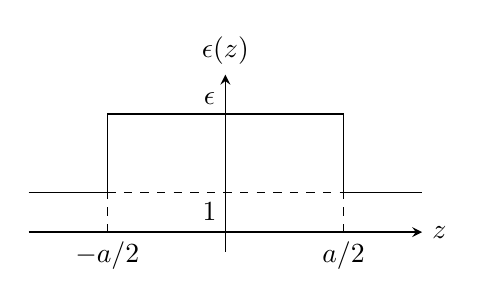
\begin{tikzpicture}[scale=.5]
      \draw[->,>=stealth,semithick](-5,0)--(5,0)node[right]{$z$};
      \draw[->,>=stealth,semithick](0,-0.5)--(0,4)node[above]{$\epsilon(z)$};
      \draw(-5,1)--(-3,1)--(-3,3)--(-0.4,3)node[above]{$\epsilon$}--(3,3)--(3,1)--(5,1);
      \draw[dashed](-3,0)node[below]{$-a/2$}--(-3,1);
      \draw[dashed](3,0)node[below]{$a/2$}--(3,1);
      \draw[dashed](-3,1)--(-0.4,1)node[below]{1}--(3,1);
    \end{tikzpicture}
    \end{figure}


    このとき、$\mathbf{H(r)} = \phi(z) e^{i k_y y} \hat{x}$であり、マスター方程式に代入すると、
    \begin{align*}
      \nabla \times  \left\{   \frac{1}{\epsilon(z)} \nabla \times (\phi(z) e^{i k_y y} \hat{x}) \right\} = \left( \frac{\omega}{c} \right)^2 \phi(z) e^{i k_y y} \hat{x}
    \end{align*}
    このとき、
    \begin{align*}
      \nabla \times \left( \phi(z) e^{ik_y y} \hat{x} \right) &= \nabla \times 
      \begin{pmatrix}
        \phi(z) e^{ik_y y} \\
        0 \\
        0 \\
      \end{pmatrix}
      = 
      \begin{pmatrix}
        0 \\
        \displaystyle \frac{d\phi}{dz}e^{ik_y y} \\
        -ik_y \phi(z) e^{ik_y y} \\
      \end{pmatrix}
    \end{align*}
    よって、
    \begin{align*}
      \nabla \times  \left\{   \frac{1}{\epsilon(z)} \nabla \times (\phi(z) e^{i k_y y} \hat{x}) \right\} &= \nabla \times \left\{ \frac{1}{\epsilon(z)} 
      \begin{pmatrix}
        0 \\
        \displaystyle \frac{d\phi}{dz}e^{ik_y y} \\
        -ik_y \phi(z) e^{ik_y y} \\
      \end{pmatrix}
      \right\}
    \end{align*}
    ここで、元の式の両辺を比較すると右辺は$x$成分しか持たないことがわかるので上式の計算結果は$y,z$成分に関しては0として良い。以下$x$成分のみの計算過程を示す。
    \begin{align*}
      &\frac{d}{dy} \left( -\frac{1}{\epsilon (z)} ik_y \phi (z) e^{ik_y y} \right) - \frac{d}{dz} \left( \frac{1}{\epsilon (z)} \frac{d \phi }{dz} e^{ik_y y} \right) = \left( \frac{ \omega }{c} \right)^2 \phi(z) e^{ik_y y}
      \\
      \Longleftrightarrow \quad &k_y^2 \frac{1}{\epsilon(z)}\phi(z)e^{ik_y y} - e^{ik_y y} \frac{d}{dz} \left( \frac{1}{\epsilon (z)} \frac{d \phi }{dz} \right) = \left( \frac{ \omega }{c} \right)^2 \phi(z) e^{ik_y y} \quad \cdots (*) 
    \end{align*}
    ここで、$z \leq - a / 2 , a / 2 \leq z \quad (=\textcircled{\scriptsize 1})$の範囲では$\epsilon(z) = 1$、$-a / 2 \leq z \leq a / 2 \quad (=\textcircled{\scriptsize 2})$の範囲では$\epsilon(z) = \epsilon$なので、それぞれの場合について考えていく。
    \begin{enumerate}
      \item[\textcircled{\scriptsize 1}のとき] \quad \\
      $\epsilon(z) = 1$である。$\displaystyle \frac{d}{dz}\frac{d \phi}{dz} = \frac{d^2\phi}{dz^2}$であり、(*)において、$e^{ik_y y}$は共通なのでそれぞれを割り、式の整理をすると
      \begin{align*}
        (*) \Longleftrightarrow k_y^2 \phi(z) - \frac{d^2 \phi(z)}{dz^2} = \left( \frac{\omega}{c} \right)^2 \phi(z)
      \end{align*}
      $\phi(z) = e^{- \kappa z}$の形であると仮定する(教科書に遠くに行くほど指数関数的に減衰すると記述があるので)と$\displaystyle \frac{d^2\phi(z)}{dz^2} = \kappa^2 \phi(z)$であるため、代入をして
      \begin{align*}
        k_y^2 e^{- \kappa z} - \kappa^2 e^{- \kappa z} = \left( \frac{\omega}{c} \right)^2 e^{-\kappa z}
      \end{align*}
      となる。なお、ここでの$\kappa$は減衰定数である。$e^{- \kappa z}$で両辺を割って
      \begin{align*}
        & k_y^2 - \kappa^2 = \left( \frac{\omega}{c} \right)^2
        \\
        \Longleftrightarrow \quad & \kappa^2 = k_y^2 - \left( \frac{\omega}{c} \right)^2
      \end{align*}
      $\kappa$は実数なので、$k_y$の満たす条件は、$k_y \geq \displaystyle \frac{\omega}{c}$である。
      \item[\textcircled{\scriptsize 2}のとき] \quad \\
      $\epsilon(z) = \epsilon$であるため、先程と同様にして
      \begin{align*}
        (*) &\Longleftrightarrow \frac{k_y^2}{\epsilon} \phi(z) - \frac{1}{\epsilon} \frac{d^2 \phi(z)}{dz^2} = \left( \frac{\omega}{c} \right)^2 \phi(z) 
        \\
        &\Longleftrightarrow \left(  \frac{k_y^2}{\epsilon}  - \left( \frac{\omega}{c} \right)^2 \right) \phi(z) = \frac{1}{\epsilon} \frac{d^2 \phi(z)}{dz^2} 
        \\
        &\Longleftrightarrow \frac{d^2 \phi(z)}{dz^2} = \left( k_y^2  - \epsilon \left( \frac{\omega}{c} \right)^2 \right) \phi(z)
      \end{align*}
      となる。

      $\phi (z) = \cos (kz), \sin (kz)$となる。$k$を求めるために$z = a / 2$における境界条件$\displaystyle \lim_{z \to a / 2 -0} \phi(z) = \lim_{z \to a / 2 + 0} \phi(z)$を考えていく。それぞれの$\phi$について考えていく。
    \end{enumerate}
      \begin{enumerate}
        \item $\phi(z) = \cos (kz)$のとき \\
        \begin{align*}
          \cos \left( \frac{ka}{2} \right) =  A e^{- \frac{\kappa a}{2}}
        \end{align*}
        もう一つの境界条件$\displaystyle \lim_{z \to -a / 2 - 0} \frac{1}{\epsilon(z)}\frac{d \phi(z)}{dz} = \lim_{z \to a / 2 + 0} \frac{1}{\epsilon(z)}\frac{d \phi(z)}{dz}$を考えていく。
        \begin{itembox}[l]{なぜ$1/\epsilon$が必要なのか}
          式(*)の両辺を$e^{ik_y y}$で割り、$a/2$を挟む形で積分を行う。つまり、
          \begin{align*}
            \int_{a/2 - \delta}^{a/2 + \delta'} \left[  k_y^2 \frac{1}{\epsilon(z)}\phi(z) - \frac{d}{dz} \left( \frac{1}{\epsilon (z)} \frac{d \phi }{dz} \right) \right]dz = \int_{a/2 - \delta}^{a/2 + \delta'} \left( \frac{ \omega }{c} \right)^2 \phi(z) dz
          \end{align*}
          ここで、$\delta, \delta' \to 0$を考えると左辺第一項と右辺は、すでに判明している境界条件から0になることがわかる。したがって、等式が成立するためには左辺第2項が0である必要がある。よって、
          \begin{align*}
            & \quad \int_{a/2 - \delta}^{a/2 + \delta'} \frac{d}{dz} \left(  \frac{1}{\epsilon (z)} \frac{d \phi }{dz} \right)dz = 0
            \\
            \Longleftrightarrow & \quad \int_{a / 2 - \delta}^{a / 2 + \delta'} d \left( \frac{1}{\epsilon (z)} \frac{d \phi }{dz} \right) = 0
            \\
            \Longleftrightarrow & \quad \left[  \frac{1}{\epsilon (z)} \frac{d \phi }{dz} \right]_{a/2 - \delta}^{a / 2 + \delta'} = 0
          \end{align*}
          以上のことから、境界条件として$\displaystyle \frac{1}{\epsilon(z)} \frac{d \phi(z)}{dz}$を考える必要があることがわかる。
        \end{itembox}
        境界条件$ \displaystyle \frac{1}{\epsilon (z)} \frac{d \phi(z)}{dz}$は、
        \begin{align*}
          \frac{k}{\epsilon} - \sin \left( \frac{ka}{2} \right) = - A \kappa e^{- \frac{\kappa a}{2}}
        \end{align*}
        したがって、以上2式を連立することにより、
        \begin{align*}
          \frac{k}{\epsilon} \tan \left( \frac{ka}{2} \right) &=  \kappa = \sqrt{k_y^2 - \left( \frac{\omega}{c} \right)^2} = \sqrt{k_y^2 - \frac{k_y^2 + k^2}{\epsilon}}
          \\
          &= \sqrt{\left( 1 - \frac{1}{\epsilon} \right)k_y^2 + \frac{k^2}{\epsilon}}
        \end{align*}
        両辺に$a$をかけて、$ka = x$とすると、
        \begin{align*}
          \frac{ka}{\epsilon} \tan \left( \frac{ka}{2} \right) &= \sqrt{\left( 1 - \frac{1}{\epsilon} \right)a^2 k_y^2 + \frac{a^2 k^2}{\epsilon}}
          \\
          \Longleftrightarrow \frac{x}{\epsilon} \tan \left( \frac{x}{2} \right) &=  \sqrt{\left( 1 - \frac{1}{\epsilon} \right)a^2 k_y^2 + \frac{x^2}{\epsilon}}
        \end{align*}

        \item $\phi(z) = \sin (kz)$のとき \\
        同様の操作を繰り返すことにより、sinの場合も導出可能である。結果は
        \begin{align*}
          \frac{x}{\epsilon} \cot \left( \frac{x}{2} \right) = - \sqrt{\left( 1 - \frac{1}{\epsilon} \right) k_y^2 a^2 - \frac{1}{\epsilon}x^2}
        \end{align*}
        になるはず。
    \end{enumerate}
    \item 第3章式(16)の各操作の説明
    
    該当する式は以下の通り。
    \begin{align*}
      \hat{T}_{\mathbf{R}}\left( \hat{O}_\mathcal{R} \mathbf{H}_{\mathbf{k}n} \right) &= \hat{O}_\mathcal{R} \left( \hat{T}_{\mathcal{R}^{-1}\mathbf{R}}\mathbf{H}_{\mathbf{k}n} \right) 
      \\
      &= \hat{O}_\mathcal{R} \left( e^{-i\left( \mathbf{k}\cdot \mathcal{R}^{-1}\mathbf{R} \right)}  \mathbf{H}_{\mathbf{k}n }\right)
      \\
      &= e^{-i \left( \mathbf{k} \cdot \mathcal{R}^{-1}\mathbf{R} \right) }\left( \hat{O}_\mathcal{R} \mathbf{H}_{\mathbf{k}n} \right)
      \\
      &= e^{-i \mathcal{R} \mathbf{k \cdot R}}\hat{O}_{\mathcal{R}} \mathbf{H}_{\mathbf{k}n}
    \end{align*}
    この操作を説明するためには並進操作と回転操作の説明が必要である。なお、$\mathbf{H}_{\mathbf{k}n}$は位置ベクトル$\mathbf{r}$を引数に持つ。
    \begin{itembox}[l]{説明}
      \begin{itemize}
        \item \textbf{回転操作}\\
        回転操作の演算子は$\hat{O}_{\mathcal{R}}$である。実際にベクトル場に作用させると、
        \begin{align*}
          \hat{O}_{\mathcal{R}} \cdot \mathbf{f(r)} = \mathcal{R}\mathbf{f}(\mathcal{R}^{-1}\mathbf{r}).
        \end{align*}
        となる。つまり、ベクトル自体と、引数を同時に$\mathcal{R}$だけ回転する操作である。
        \\
        (教科書第3章式(14)参照)
        \item \textbf{並進操作}\\
        並進操作の演算子は$\hat{T}_{\mathbf{R}}$である。実際に作用させると、
        \begin{align*}
          \hat{T}_{\mathbf{R}} \epsilon(\mathbf{r}) = \epsilon(\mathbf{r} - \mathbf{R})
        \end{align*}
        となる。
        \\
        (教科書第3章式(4)付近を参照)
      \end{itemize}
    \end{itembox}
    以上のことを踏まえて各行ごとの操作を説明する。
    \begin{itemize}
      \item[1行目.] $\mathbf{H}_{\mathbf{k}n}$に対して、回転操作を行う。つまり、
      \begin{align*}
        \hat{T}_{\mathbf{R}}\left( \hat{O}_{\mathcal{R}} \mathbf{H}_{\mathbf{k}n} \left( \mathbf{r} \right) \right) = \hat{T}_\mathbf{R} \left( \mathcal{R} \mathbf{H}_{\mathbf{k}n} \left( \mathcal{R}^{-1} \mathbf{r} \right) \right)
      \end{align*}
      ここで、並進演算子を作用させると、
      \begin{align*}
        \hat{T}_\mathbf{R} \left( \mathcal{R} \mathbf{H}_{\mathbf{k}n} \left( \mathcal{R}^{-1} \mathbf{r} \right) \right) = \mathcal{R} \mathbf{H}_{\mathbf{k}n} \left( \mathcal{R}^{-1} \left( \mathbf{r} - \mathbf{R} \right) \right)
      \end{align*}
      この式は、\textbf{$\mathbf{H}$に対して、} $\hat{T}_{\mathcal{R}^{-1} \mathbf{R}}$ \textbf{を作用させ、回転演算子$\hat{O}_\mathcal{R}$を作用させたもの}として見ることができる。
      よって、
      \begin{align*}
        \hat{T}_{\mathbf{R}}\left( \hat{O}_{\mathcal{R}} \mathbf{H}_{\mathbf{k}n}  \right) = \hat{O}_\mathcal{R} \left( \hat{T}_{\mathcal{R}^{-1}\mathbf{R}}\mathbf{H}_{\mathbf{k}n} \right)
      \end{align*}
      \item[2行目.] 関数$\mathbf{H_k} = \mathbf{H_0}e^{i\mathbf{k \cdot r}}$に対して、回転操作を行っているので、$\hat{T}_{\mathcal{R}^{-1}\mathbf{R}}$は$e^{-i\mathbf{k \cdot \mathcal{R}^{-1}\mathbf{R}}}$に変化している。
      \item[3行目.] $e^{-i\mathbf{k \cdot \mathcal{R}^{-1}\mathbf{R}}}$は回転演算子$\hat{O}$の影響を受けない(定数だから)。よって順番を並び替えただけ
      \item[4行目.] $e$の肩に乗っている2つのベクトル$\mathbf{k, R}$を$\mathcal{R}$だけ回転している。ベクトルの内積は2つのベクトルの大きさ同士の積に成す角のcosをかけたものであるため、2つのベクトル両方を同じ角度だけ回転させた場合、内積は不変である。よって、
      \begin{align*}
        \mathbf{k} \cdot \mathcal{R}^{-1} \mathbf{R} = \mathcal{R} \mathbf{k} \cdot \mathbf{R}
      \end{align*}
      となるため、式のような変形が可能である。
    \end{itemize}

  \item 2つの異なる屈折率で構成されたフォトニック結晶を考える
  
  
  $0 \leq z \leq b$のときに屈折率$\epsilon_1$、$b \leq z \leq a$のときに屈折率$\epsilon_2$で周期$a$で繰り返される結晶を考える。このとき、$\mathbf{u} (z) = \mathbf{u} (z + R)$($R$は$a$の整数倍)が成立する。(*)に代入すると、$k_y = 0$だから、
    \begin{align*}
      (*) &\Longleftrightarrow - \frac{d}{dz}\left( \frac{1}{\epsilon(z)} \frac{d\phi}{dz} \right) = \left( \frac{\omega}{c} \right)^2 \phi(z)
      \\
      \phi (z) &= 
      \begin{cases}
        \phi_1 = A e^{ik_1 z} + B e^{- i k_1 z} \quad \left( 0 \leq z \leq b \right) \\
        \phi_2 = C e^{ik_2 z} + D e^{- i k_2 z} \quad \left( b \leq z \leq a \right)
      \end{cases}
    \end{align*}

    となる。接続条件を考えると

    \begin{align*}
      & A e^{i k_1 b} + B e^{- i k_1 b} = C e^{i k_2 b} + D e^{- i k_2 b}
      \\
      & \frac{A k_1}{\epsilon_1} e^{i k_1 b} - \frac{B k_1}{\epsilon_1} e^{- i k_1 b} = \frac{C k_2}{\epsilon_2} e^{i k_2 b} - \frac{D k_2}{\epsilon_2}e^{- i k_2 b}
    \end{align*}

    となる。この2つの式から、$C, D$を$A, B$で表すと
    \begin{align*}
      C &= \frac{1}{2} \left\{ \left( \alpha + 1 \right) A e^{i \left( k_1 - k_2 \right) b } + \left( 1 - \alpha \right) B e^{- i \left( k_1 + k_2 \right) b } \right\} \\
      D &= \frac{1}{2} \left\{ \left( \alpha - 1 \right) A e^{i \left( k_1 + k_2 \right) b} + \left( 1 + \alpha \right) B e^{- i (k_1 - k_2)b} \right\}
    \end{align*}
    となる。なお、ここで$\displaystyle \frac{k_1 \epsilon_1}{k_2 \epsilon_2} = \sqrt{\frac{\epsilon_2}{\epsilon_1}} = \alpha$とした。$\left( \displaystyle k_i = \sqrt{\epsilon_i} \frac{\omega}{c}  に注意 \right) $

    次に、$z = a$の時を考える。このとき、$\phi(a) = e^{i k_z a} \phi (0)$である($k_z$はブロッホ波数)。接続条件は、
    \begin{align*}
      & e^{i k_z a} (A + B) = C e^{i k_2 a} + D e^{- i k_2 a} \\
      & \alpha (A - B) e^{i k_z a} = C e^{i k_z a} - D e^{- i k_z a}
    \end{align*}
    以上の式を$C, D$を削除し、$A, B$に関する式にする。
    \begin{align*}
      (A + B) e^{i k_z a} = & \frac{1}{2} \left\{ \left( \alpha + 1 \right) A e^{i \left( k_1 - k_2 \right) b } + \left( 1 - \alpha \right) B e^{- i \left( k_1 + k_2 \right) b } \right\} e^{i k_2 a} 
      \\ + & \frac{1}{2} \left\{ \left( \alpha - 1 \right) A e^{i \left( k_1 + k_2 \right) b} + \left( 1 + \alpha \right) B e^{- i (k_1 - k_2)b} \right\} e^{- i k_2 a} 
    \end{align*}
    \begin{align*}
      \alpha (A - B) e^{i k_z a} = & \frac{1}{2} \left\{ \left( \alpha + 1 \right) A e^{i \left( k_1 - k_2 \right) b } + \left( 1 - \alpha \right) B e^{- i \left( k_1 + k_2 \right) b } \right\} e^{i k_2 a} 
      \\ - & \frac{1}{2} \left\{ \left( \alpha - 1 \right) A e^{i \left( k_1 + k_2 \right) b} + \left( 1 + \alpha \right) B e^{- i (k_1 - k_2)b} \right\} e^{- i k_2 a}
    \end{align*}
    2つの式から行列式を求めると、
    \begin{align*}
      (1 + \alpha)^2 \left( e^{i (k_z - k_2)a} - e^{i(k_z - k_2)b} \right) \left( e^{i (k_z + k_2)a} - e^{- i(k_1 - k_2)b} \right) = 0
    \end{align*}
    展開し、両辺を$e^{i k_z a}$で割ると、
    \begin{align*}
      \cos k_z a &= \frac{1}{4 \alpha} \left\{ (1 + \alpha)^2 \cos \left( k_2 a + k_1 b - k_2 b \right) - (1 - \alpha)^2 \cos \left( k_2 a - k_1 b - k_2 \right) \right\} 
      \\
      &= \frac{1}{4 \alpha} (1 + \alpha^2) \left\{ \cos \left( k_2 a + k_1 b - k_2 b \right) - \cos \left( k_2 a - k_1 b - k_2 b \right) \right\} 
      \\
      &\quad + \frac{1}{2} \left\{ \cos \left( k_2 a + k_1 b - k_2 b \right) + \cos \left( k_2 a - k_1 b - k_2 b \right) \right\} 
      \\
      &= \frac{1 + \alpha^2}{4 \alpha} \left[ -2 \sin \left\{ k_2 \left( a - b \right) \right\} \sin k_1 b \right] + \frac{1}{2} \left[ 2 \cos \left\{ k_2 \left( a - b \right) \right\} \cos k_1 b \right]
      \\
      &= - \frac{1}{2} \left( \alpha + \frac{1}{\alpha} \right) \sin \left\{ k_2 \left( a - b \right) \right\} \sin (k_1 b) + \cos \left\{ k_2 \left( a - b \right) \right\} \cos (k_1 b)
    \end{align*}
    ここで、$a - b, b$は結晶の厚さを表しており、それぞれの領域における波数$k$と対応している。$\alpha \neq 1$では$| \cos k_z a | > 1$となり、バンドギャップが生成される。

    $b = 0.5a$とし、分散関係を用いて式を整理すると
    \begin{align*}
      - \frac{1}{2} \left( \alpha + \frac{1}{\alpha} \right) \sin \left( \sqrt{\epsilon_2} \frac{\omega a}{2 c} \right)\sin \left( \sqrt{\epsilon_1} \frac{\omega a}{2 c} \right) + \cos \left( \sqrt{\epsilon_2} \frac{\omega a}{2 c} \right)\cos \left( \sqrt{\epsilon_1} \frac{\omega a}{2 c} \right)
    \end{align*}
    $\displaystyle \frac{\omega a}{2 \pi c} = x$とすると、
    \begin{align*}
      - \frac{1}{2} \left( \alpha + \frac{1}{\alpha} \right) \sin \left( \sqrt{\epsilon_2} \pi x \right)\sin \left( \sqrt{\epsilon_1} \pi x \right) + \cos \left( \sqrt{\epsilon_2} \pi x \right)\cos \left( \sqrt{\epsilon_1} \pi x \right)
    \end{align*}
    この式が$-1$となるときにバンドギャップを与える。そこからミッドギャップ周波数が決まる。
    \item 教科書第4章式(2)の導出
    \begin{align*}
      \frac{\Delta \omega}{\omega_m} \thickapprox \frac{\Delta \epsilon}{\epsilon} \frac{\sin \pi d / a}{\pi}
    \end{align*}
    \begin{proof}[導出]
      条件として、$\displaystyle \frac{\Delta \epsilon}{\epsilon} \ll 1$もしくは $\displaystyle \frac{d}{a}$が十分に小さいがある。 
    \end{proof}
    \item 以下の2つの項目に関して説明せよ
    \begin{itemize}
      \item[(1).] 導波管を伝わるモードはどのようにして記述できるか
      \item[(2).] 長方形の横を取っ払って金属でサンドイッチされた状態でカットオフ周波数が生じない理由(電場接線方向を向いているか垂直を向いてるか)
    \end{itemize}
    \textbf{説明}
    \\
    TEモード、TMモードはそれぞれ以下のように説明される
      \begin{itemize}
        \item[-] TE(Transverse Electric)モード:\textcolor{red}{電場}が導波管の伝搬方向に垂直
        \item[-] TM(Transverse Magnetic)モード:\textcolor{red}{磁場}が導波管の伝搬方向に垂直
      \end{itemize}
    \begin{itemize}
      \item[(1).] 波が$z$方向に伝搬し、$x$方向の幅が$a$、$y$方向の幅が$b$の短形導波管を考える。このとき、カットオフ周波数$\omega_c$は以下のようにして記述される。
      \begin{align*}
        \omega_c = c \sqrt{\left( \frac{n \pi}{a} \right)^2 + \left( \frac{m \pi}{b} \right)^2} \quad (c:光速、 n: x方向の波の数、m:y方向の波の数)
      \end{align*}
      
      \item[(2).] カットオフ周波数とは、\textbf{導波管で伝送することが可能な最低周波数}のこと(つまり最大波長)。
      なので、長方形の横を取っ払って金属でサンドイッチされた状態でカットオフ周波数が生じないのは横方向への制限がなくなり、
    \end{itemize}
    \item fcc格子のブリルアンゾーンがなぜ教科書に掲載されているような形となっているのか説明せよ
      \\ 
      fcc格子の基本並進ベクトルは以下の3つである
      \begin{align*}
        \boldsymbol{a}_1 = \frac{a}{2}\begin{pmatrix} 1 \\ 1 \\ 0\end{pmatrix}, 
        \boldsymbol{a}_2 = \frac{a}{2}\begin{pmatrix} 1 \\ 0 \\ 1\end{pmatrix}, 
        \boldsymbol{a}_3 = \frac{a}{2}\begin{pmatrix} 0 \\ 1 \\ 1\end{pmatrix}
      \end{align*}
      したがって逆格子ベクトルを求めると、
      \begin{align*}
        \boldsymbol{b}_1 = \frac{2 \pi}{a} \begin{pmatrix}1 \\ 1 \\ -1\end{pmatrix}, 
        \boldsymbol{b}_2 = \frac{2 \pi}{a} \begin{pmatrix}-1 \\ 1 \\ 1\end{pmatrix}, 
        \boldsymbol{b}_3 = \frac{2 \pi}{a} \begin{pmatrix}1 \\ -1 \\ 1\end{pmatrix}
      \end{align*}
      となる。以上のことから逆格子ベクトル$\boldsymbol{G}$は整数$l, m, n$を用いて以下のように書くことができる。
      \begin{align*}
        \boldsymbol{G} = l \boldsymbol{b}_1 + m \boldsymbol{b}_2 + n \boldsymbol{b}_3
      \end{align*}
      逆格子ベクトルを図示してどれか1つの軸に沿って90°ずつ回転させると以下の8つの座標を得る
      \begin{align*}
        \begin{cases}
          (1, 1, -1) \quad (l = 1, m = n = 0) \\
          (1, -1, -1) \quad (m = -1, l = n = 0) \\
          (-1, -1, -1) \quad (l = m = n = -1) \\
          (-1, 1, -1) \quad (n = -1, l = m = 0) \\
          (1, 1, 1) \quad (l = m = n = 1) \\
          (1, -1, 1) \quad (n = 1, l = m = 0) \\
          (-1, 1, 1) \quad (m = 1, l = n = 0) \\
          (-1, -1, 1) \quad (l = -1, m = n = 0) 
        \end{cases}
      \end{align*}
      以上から最近接面を求めることができた。このときの原点からの距離は$\displaystyle \frac{2\pi}{a} \sqrt{3}$である。
      
      また、ブリルアンゾーンは$x, y, z$軸方向にも面を持っていることがわかる。よって、$(\pm 1, 0, 0), (0, \pm 1, 0), (0, 0, \pm 1)$となるような係数$l, m, n$を考えてみる。例として$(1, 0, 0)$の場合
      \begin{align*}
        l - m + n &= 1 \\
        l + m - n &= 0 \\
        -l + m + n &= 0 
      \end{align*}
      以上を解くと、$(l, m, n) = (1/2, 0, 1/2)$となる。$l, m, n$は整数であることからすべての式を2倍すれば良く、このときの原点からの距離は$\displaystyle \frac{4\pi}{a}$である。
      以上のことからfcc格子のブリルアンゾーンは教科書に掲載されているような形となる。
    \item ヤブロノバイトの棒がどうして教科書のような形になっているのか。
      \begin{itemize}
        \item (111)面の法線と棒のなす角が35.26degである理由
        \begin{proof}
          fcc格子の基本並進ベクトルは以下の3つである。
          \begin{align*}
            \boldsymbol{a}_1 = \frac{a}{2}\begin{pmatrix} 1 \\ 1 \\ 0\end{pmatrix}, 
            \boldsymbol{a}_2 = \frac{a}{2}\begin{pmatrix} 1 \\ 0 \\ 1\end{pmatrix}, 
            \boldsymbol{a}_3 = \frac{a}{2}\begin{pmatrix} 0 \\ 1 \\ 1\end{pmatrix}
          \end{align*}
          また面(111)の法線ベクトルは、$\begin{pmatrix}1 \\ 1 \\ 1\end{pmatrix}$なので、2つのベクトルのなす角はそれぞれのベクトルの大きさと内積からもとめる事ができる。1例として、$\displaystyle \frac{a}{2}\begin{pmatrix} 1 \\ 1 \\ 0\end{pmatrix}$とのなす角について述べる。なす角を$\theta$とすると、
          \begin{align*}
            \cos \theta = \frac{ \boldsymbol{a \cdot b} }{| \boldsymbol{a} | | \boldsymbol{b} |} = \cfrac{a}{\cfrac{a}{\sqrt{2}} \sqrt{3}} = \sqrt{\frac{2}{3}} \quad \therefore \theta \simeq 35.26 \mathrm{deg}
          \end{align*}
          となることがわかる。
        \end{proof}
        \item なぜ棒が120°ずつ分布しているのか
          \begin{proof}
            これは言い換えると、3つの基本並進ベクトルを(111)面に射影したもののなす角が120°になる理由を答えよということ。
            
            並進ベクトルは整数$l, m, n$を用いることで以下のようにして書くことができる。
            \begin{align*}
              \boldsymbol{R} = l \boldsymbol{a_1} + m \boldsymbol{a_2} + n \boldsymbol{a_3} = \frac{1}{2}
              \begin{pmatrix}
                l + n \\
                l + m \\
                m + n
              \end{pmatrix}
            \end{align*}
            このとき、$R$を(111)面の法線ベクトルと平行な成分と垂直な成分に分けて書きたい。

            よって、$\boldsymbol{R} = \boldsymbol{R}_{\parallel} + \boldsymbol{R}_{\perp}$のようにしてそれぞれの成分に分ける。また、法線ベクトルを規格化したものとして$\boldsymbol{n} = 1 / \sqrt{3} (1, 1, 1)$を定義する。このとき、$\boldsymbol{R}_{\parallel}$は$\boldsymbol{n}$と平行なので実数$\alpha$を用いて$\boldsymbol{R}_{\parallel} = \alpha \boldsymbol{n}$と書けることがわかる。

            以下で$\alpha$を求めていく。
            \begin{gather*}
              \boldsymbol{R}_{\parallel} = \alpha \boldsymbol{n} \\
              \boldsymbol{n} \cdot \boldsymbol{R}_{\parallel} = \alpha \boldsymbol{n} \cdot \boldsymbol{n} = \alpha |\boldsymbol{n}|^2  \\
              \boldsymbol{n} \cdot \boldsymbol{R} = \alpha \quad ( \because |\boldsymbol{n}| = 1 )
            \end{gather*}
            最終行において、$\boldsymbol{n} \cdot \boldsymbol{R}_{\parallel} = \boldsymbol{n} \cdot \boldsymbol{R}$としたのは、$\boldsymbol{R}$を$\boldsymbol{n}$と平行成分と垂直成分に分けて、垂直なベクトルの内積が0となる性質を用いた。

            計算を実施して、
            \begin{align*}
              \alpha = 
                \frac{1}{\sqrt{3}} \begin{pmatrix} 1 \\ 1 \\ 1 \end{pmatrix} 
                \cdot \frac{1}{2} \begin{pmatrix} l + n \\ l + m \\ m + n \end{pmatrix}
                = \frac{1}{2 \sqrt{3}} \left( l + m + n \right)
            \end{align*}
            $\alpha$を求めることができたので法線ベクトルに垂直な成分を求めていく。
            \begin{align*}
              \boldsymbol{R}_{\perp} &= \boldsymbol{R} - \boldsymbol{R}_{\parallel} = 
                \frac{a}{2} \begin{pmatrix}l + m \\ l + n \\ n + m\end{pmatrix} 
                - \frac{1}{3} \begin{pmatrix}l + m + n \\ l + m + n  \\ l + m + n \end{pmatrix}
                \\
                &= \frac{1}{6}\begin{pmatrix}l + m - 2n \\ l + n - 2m \\ n + m - 2l\end{pmatrix}
                = \frac{l}{6}\begin{pmatrix}1 \\ 1 \\ -2 \end{pmatrix} + \frac{m}{6}\begin{pmatrix}1 \\ -2 \\ 1 \end{pmatrix} + \frac{n}{6}\begin{pmatrix}-2 \\ 1 \\ 1 \end{pmatrix}
            \end{align*}
            ここで、$l, m , n$にかかるベクトルをそれぞれ$\hat{\boldsymbol{x}'}, \hat{\boldsymbol{y}'}, \hat{\boldsymbol{z}'}$、とする。このとき、$\hat{\boldsymbol{x}'} + \hat{\boldsymbol{y}'} = - \hat{\boldsymbol{z}'}$が成立する。よって、$\boldsymbol{R}_{\perp}$を$\hat{\boldsymbol{x}'}, \hat{\boldsymbol{y}'}$で表すと、
            \begin{align*}
              \boldsymbol{R}_{\perp} = \frac{l - n}{6} \hat{\boldsymbol{x}'} + \frac{m - n }{6} \hat{\boldsymbol{y}'}
            \end{align*}
            となる。$\hat{\boldsymbol{x}'}$と$\hat{\boldsymbol{y}'}$のなす角は、120°だから(111)面に射影すると120°ずつ分布し、三角格子となる。
          \end{proof}
      \end{itemize}
      \item $y$方向に有限の幅($0.4a$)を持つ帯を伝搬する電磁波を考える。$xy$平面上を伝搬するTMモードを考える。つまり、$k_z = 0であり、 E_z$成分のみを持つ。
        この時、成立する条件として、$\nabla \cdot \mathbf{H}=0$が成立する。また、帯の外で$y$方向の波は指数関数的に減衰していく。

        この時、磁場は波数に垂直な方向を向いた磁場の平面波の重ね合わせで書く必要がある。よって、以下のように書ける。
        \begin{align*}
          \mathbf{H}_1 &= e^{i(k_x x + k_y y)}(H_x \hat{\boldsymbol{x}} + H_y \hat{\boldsymbol{y}}) \\
          \mathbf{H}_2 &= e^{i(k_x x - k_y y)}(H_x' \hat{\boldsymbol{x}} - H_y' \hat{\boldsymbol{y}}) 
        \end{align*}
        条件$\nabla \cdot \mathbf{H}=0$を以上の2つの式に適用することで、以下の2つが得られる。
        \begin{align*}
          k_x H_x + k_y H_y &= 0 \quad \cdots (1) \\
          k_x H_x' - k_y H_y' &= 0 \quad \cdots (2)
        \end{align*}
        帯内の磁場は$\mathbf{H}_1$と$\mathbf{H}_2$の線形結合で書けるので、
        \begin{align*}
          \mathbf{H} = \alpha \mathbf{H}_1 + \beta \mathbf{H}_2 = e^{ik_x x} \left\{ (\alpha e^{ik_y y} H_x + \beta e^{- i k_y y} H_x' ) \hat{\boldsymbol{x}}  + (\alpha e^{ik_y y} H_y + \beta e^{- i k_y y} H_y' ) \hat{\boldsymbol{y}}\right\}
        \end{align*}
        $y$依存性は、システムの依存性からsinもしくは、cosの形で掛ける必要がある。よって、$\alpha H_x$などは任意の値を取ることができない。

        $\alpha H_x = \beta H_x'$が成立する時、$x$成分はcosでかけて、$y$成分はsinでかけることができる。よって、これを適用すると
        \begin{align*}
          \mathbf{H} = e^{i k_x x} \left\{ 2 \alpha H_x \cos \left( k_y y \right) \hat{\boldsymbol{x}} + 2 i \alpha H_y \sin \left( k_y y \right) \hat{\boldsymbol{y}} \right\}
        \end{align*}
        となる。

        次に、帯の外側を考える。はじめに帯を上側を考える。$y$は指数関数的に減衰するため、減衰定数を$\kappa$とすると、
        \begin{align*}
          \mathbf{H} = e^{i k_x x - \kappa y}\left( H_x'' \hat{\boldsymbol{x}} + H_y'' \hat{\boldsymbol{y}} \right)
        \end{align*}
        と書ける。$y$方向への対称性(偶関数か奇関数か)で$\kappa$の符号が入れ替わる。条件$\nabla \cdot \mathbf{H}$を考えると、
        \begin{align*}
          i k_x H_x'' - \kappa H_y'' = 0 \quad \cdots (3) \\
        \end{align*}
        となる。次に磁場の接続を考える。帯の$y$方向の幅を$w$として、中心が$y = 0$にあるとする。つまり、$y = \pm w / 2$で磁場が連続であるときの場合を考える。
        $y = w / 2$のとき、$x成分とy$成分それぞれについて考えると、
        \begin{align*}
          2 \alpha \cos \left( k_y \frac{w}{2} \right)H_x &= e^{- \kappa \frac{w}{2}} H_x'' \quad \cdots (4) \\
          2 \alpha i \sin \left( k_y \frac{w}{2} \right)H_y &= e^{- \kappa \frac{w}{2}} H_y'' \quad \cdots (5)
        \end{align*}
        $(5)/(4)$をして整理をすると、
        \begin{align*}
          \kappa = - k_y \cot \left( k_y \frac{w}{2} \right)
        \end{align*}
        $(4)/(5)$をして整理をすると、
        \begin{align*}
          \kappa = k_y \tan \left( k_y \frac{w}{2} \right)
        \end{align*}
        分散関係より、以下の等式が成立する
        \begin{gather*}
          \left( \frac{\omega}{c} \right)^2 = k_x^2 - \kappa^2
          \\
          \Longleftrightarrow  
          \kappa = \sqrt{k_x^2 - \left( \frac{\omega}{c} \right)^2} = \sqrt{k_x^2 - \frac{1}{\epsilon}(k_x^2 + k_y^2)} = \sqrt{\left( 1 - \frac{1}{\epsilon} \right) k_x^2 - \frac{k_y^2}{\epsilon}}
        \end{gather*}
        これを先の式に代入をして
        \begin{align*}
          k_y \tan \left( k_y \frac{w}{2} \right) = \sqrt{\left( 1 - \frac{1}{\epsilon} \right) k_x^2 - \frac{k_y^2}{\epsilon}}
        \end{align*}
        この式の$k_y$を変数としてグラフの交点から該当する$k_x$を求めることができる。
    \end{enumerate}
    
\end{document}